\section{User Interface}

Für das User-Interface wurde das JavaScript-Framework Angular verwendet. 
Diese Entscheidung wurde getroffen, da Angular über eine sehr umfassende 
Dokumentation verfügt und sich hervorragend für die Entwicklung von 
Webanwendungen eignet. Zudem verfügten die Teammitglieder über die meisten 
Erfahrungen mit diesem Framework, was die Entwicklung und Zusammenarbeit 
erleichterte. \newline

\noindent In JavaScript besteht die Möglichkeit, 
Pakete von anderen Entwicklern zu nutzen. Diese Pakete können mithilfe eines 
Paket-Managers wie \textit{npm} installiert werden. Im Rahmen dieses Projekts 
haben wir das Design-Framework \textit{Project Clarity} und das 
Chart-Framework \textit{chart.js} über \textit{npm} installiert.
Eine ausführlichere Betrachtung des Designs erfolgt im entsprechenden Abschnitt. \newline

\noindent Das User-Interface ist in verschiedene Seiten unterteilt. 
Eine detaillierte Betrachtung der einzelnen Seiten erfolgt im Abschnitt \textit{Seiten}. 
Die allgemeine Navigationsstruktur wird im Abschnitt \textit{Navigation} ausführlich erläutert.

\notebox {
  Für die prototypische Entwicklung wurde das User-Interface in Englischer Sprache
  entwickelt. Für die finale Version des User-Interfaces ist eine übersetzung in
  verschiedene Sprachen notwendig um eine größere Nutzergruppe zu erreichen.
  Dabei können Paktete wie \textit{ngx-translate} verwendet werden.
}

\subsection{Design}

Um die Entwicklung des User-Interfaces zu vereinfachen, wurde das Design-Framework
\textit{Project Clarity} verwendet. Dieses Framework bietet eine Vielzahl von
vorgefertigten Komponenten, die sich einfach in das User-Interface integrieren lassen.

\notebox {
  Für die prototypische Entwicklung des User-Interfaces wurde das Design-Framework
  \textit{Project Clarity} verwendet. Für die finale Version des User-Interfaces
  ist eine Anpassung des Designs an das Corporate Design der Hochschule notwendig
  um eine gleichbleibende Nutzererfahrung zu gewährleisten.
}

\noindent Für das Anzeigen von Diagrammen wurde das Chart-Framework \textit{chart.js} verwendet.
Dieses Framework bietet eine Vielzahl von Diagrammtypen, die sich einfach in das
User-Interface integrieren lassen. Diese Diagramme sind auf dem User-Dashboard 
und dem Team-Dashboard eingebunden.

\subsection{Navigation}

Die Navigation des User-Interfaces ist in zwei Bereiche unterteilt. 
Der erste Bereich ist die Navigationsbar, die sich am oberen Rand des User-Interfaces befindet.
In dieser Navigationsbar befinden sich die Links zu den verschiedenen Seiten des User-Interfaces,
wie User-Dashboard und Team- und Quiz-Übersicht. Zudem befindet sich in der Navigationsbar
ein Link zum User-Profil und ein Link zum Logout.

\begin{figure}[H]
  
\includegraphics[width=\linewidth]{img/navbar.png}
  \caption{Navigationsbar}
  \label{fig:navbar}
\end{figure}

Der zweite Bereich der Navigation ist die Suchbar in der oberen Navigationsbar. 
Dort kann über eine Volltextsuche nach Teams und Quizzes gesucht werden und 
direkt auf diese zugegriffen werden.

\begin{figure}[H]
  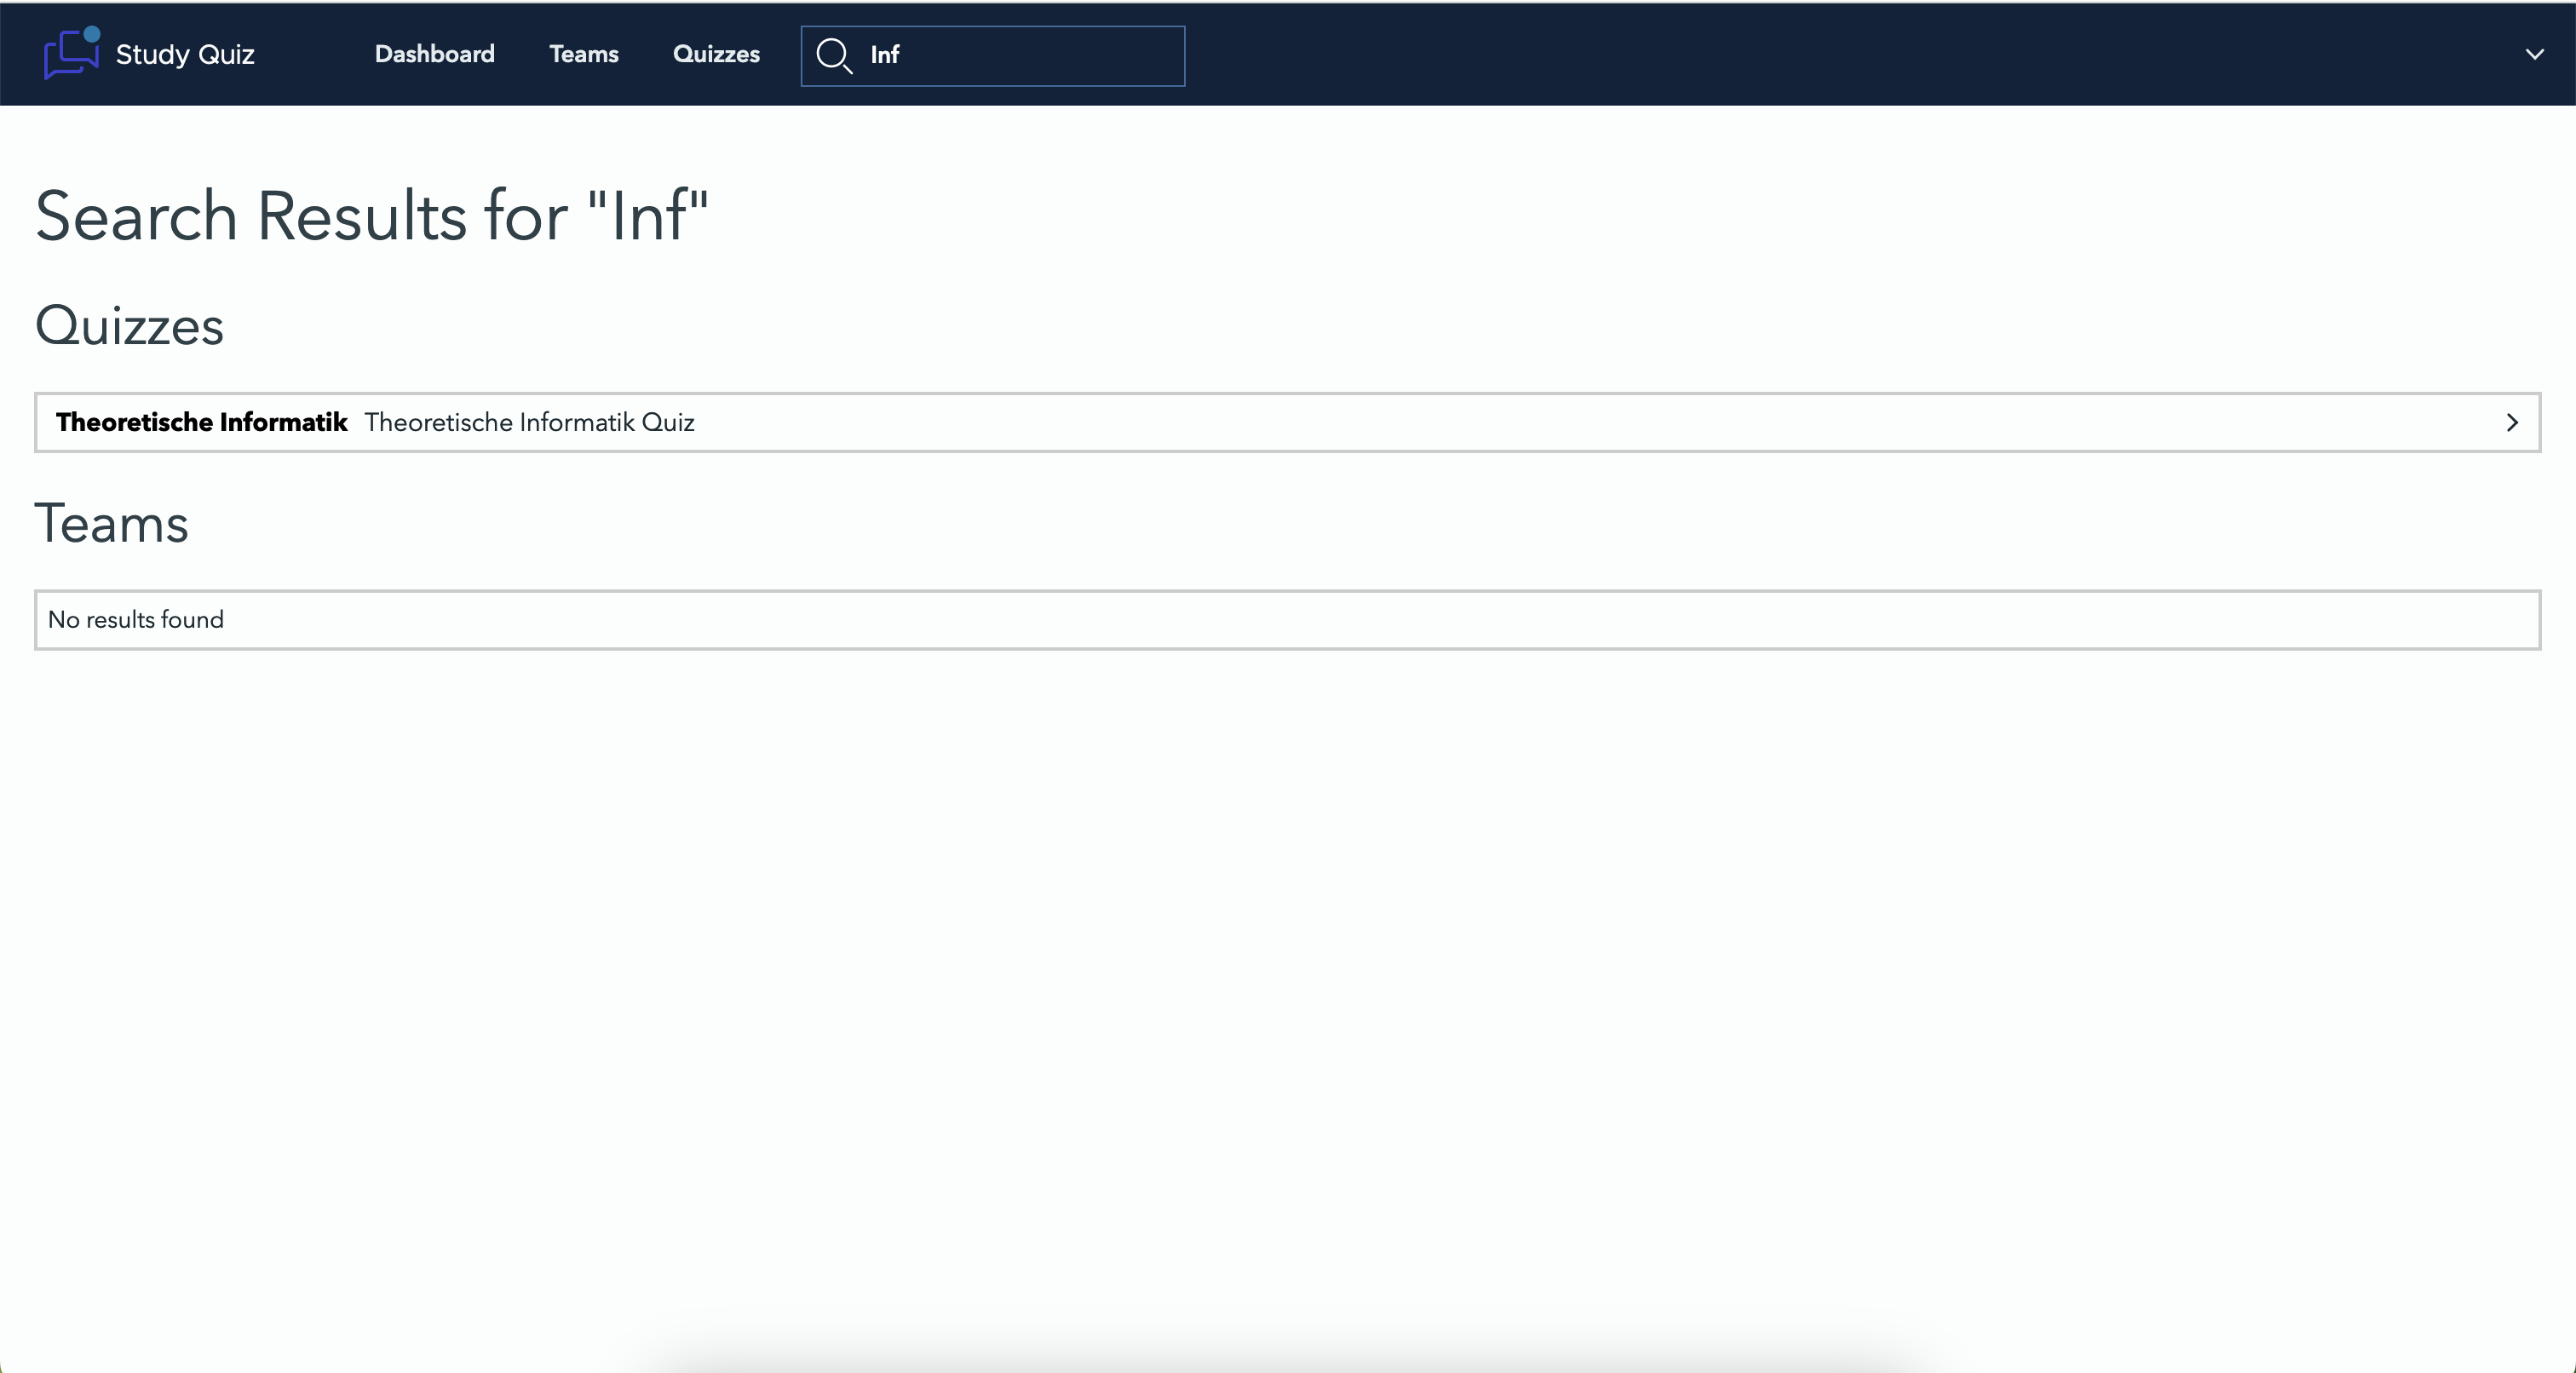
\includegraphics[width=\linewidth]{img/suche.png}
  \caption{Search-Page}
  \label{fig:searchbar}
\end{figure}
\subsection{Seiten}

\subsection*{Login \& Registrierung}

Die Login Seite bietet dem User die möglich sich am System anzumelden. 
An der linken Seite der Login Seite kann der Nutzer sein Benutzernamen
und Passwort eintragen. Wenn diese korrekt sind seir eine bestätigt angezeigt
und der User nach zwei Sekunden zum User Dashboard weitergeleitet. \newline

\noindent Wenn ein Nutzer auf eine Route der Webanwendung zufreift ohne angemeldet
zu sein, wird er automatisch auf die Anmeldenseite weitergeleitet.

\begin{figure}[H]
  
\includegraphics[width=\linewidth]{img/login.png}
  \caption{Login Seite}
  \label{fig:login}
\end{figure}

Über den unteren Limk auf der Login Seite kann ein Nutzer ohne Benutzerkonto auf die 
Anmelde-Seite gelangen. Dort muss er im Formular seinen gewünschte Benutzernamen, 
E-Mail Adresse und Passwort eingeben. Sobald das Formular valide ist kann der 
Register-Button gedrückt werden. Bei erfolgreicher Registrierung dir dem Nutzer 
eine bestätigt angezeigt und nach zwei Sekunden auf die Anmelde-Seite weitergeleitet,
wo er sich mit seinem neu erstellen Nutzerkonto anmelden kann.

\begin{figure}[H]
  
\includegraphics[width=\linewidth]{img/register.png}
  \caption{Registrierungs Seite}
  \label{fig:register}
\end{figure}

\subsection*{Dashboard}

Das Nutzer-Dashboard ist die personalisierte Seite für den Nutzer.
Es ist die Seite, welche direkt nach der Anmeldung dem Nutzer angezeigt wird. \newline

\noindent Im oberen Bereich wird dem User auf der linken Seite, den aktuellen Score von diesem
Monat angezeigt. Dieser Zählt die erreichten Punkte im Quiz für den aktuell Monat. 
Auf der rechten Seite kann der Nutzer in einem Graph seine monatlichen Punktzahlen der letzten
Monate analysieren.\newline

\noindent Im mittleren Bereich des Dashboards kann der Nutzer seine letzten 10 durchgeführten
Quizze sehen. Sollte er davon ein Quiz nicht abgeschlossen haben kann er es über einen klick auf
das Quiz fortsetzen. \newline

\noindent Im unteren Bereich des Dashboards befinden sich der Leaderboard-Bereich. 
Dort wird auf der linken Seite die zehn Nutzer mit den meisten Punkten diesen Monat angezeigt.
Auf der rechten Seite werden die zehn Teams mit den meisten Punkten diesen Monat angezeigt. \newline

\noindent Das Nutzer-Dashboard kann über den Navigationsbar über den Punkt Dashboard von
jeder Seite der Webanwendung erreicht werden.

\begin{figure}[H]
  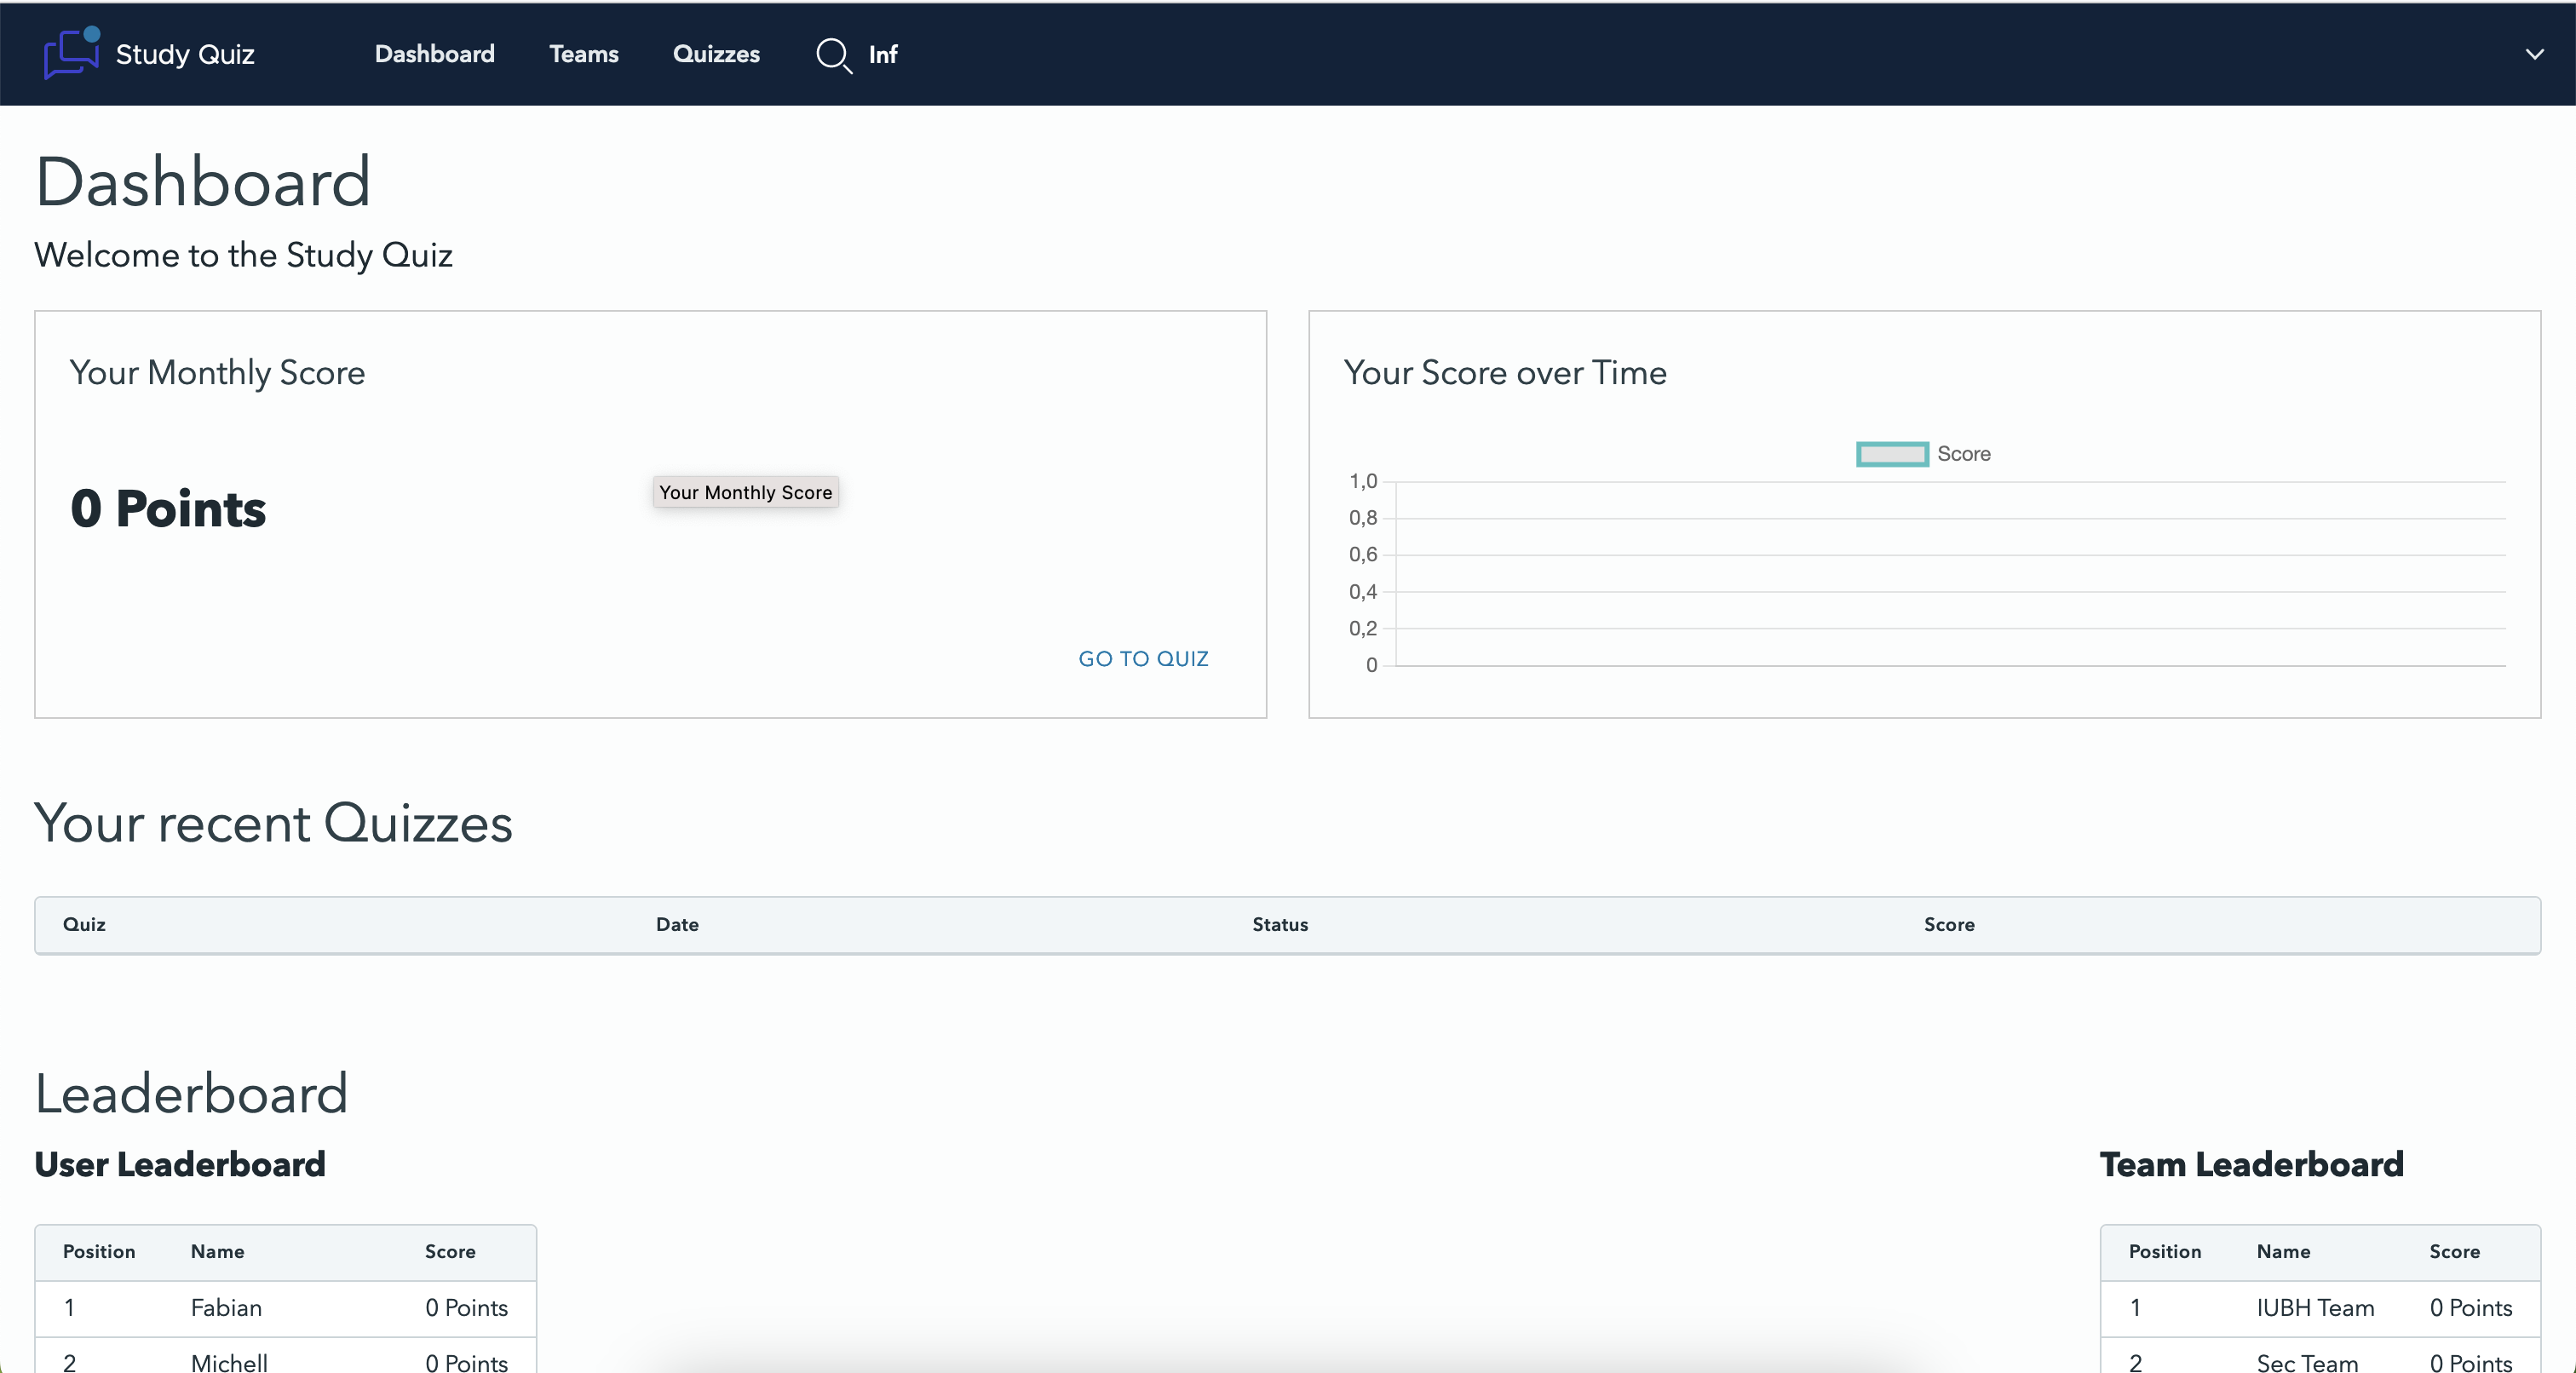
\includegraphics[width=\linewidth]{img/dashboard.png}
  \caption{Dashboard Seite}
  \label{fig:dashboard}
\end{figure}

\subsection*{Quiz Seiten}




\begin{figure}[H]
  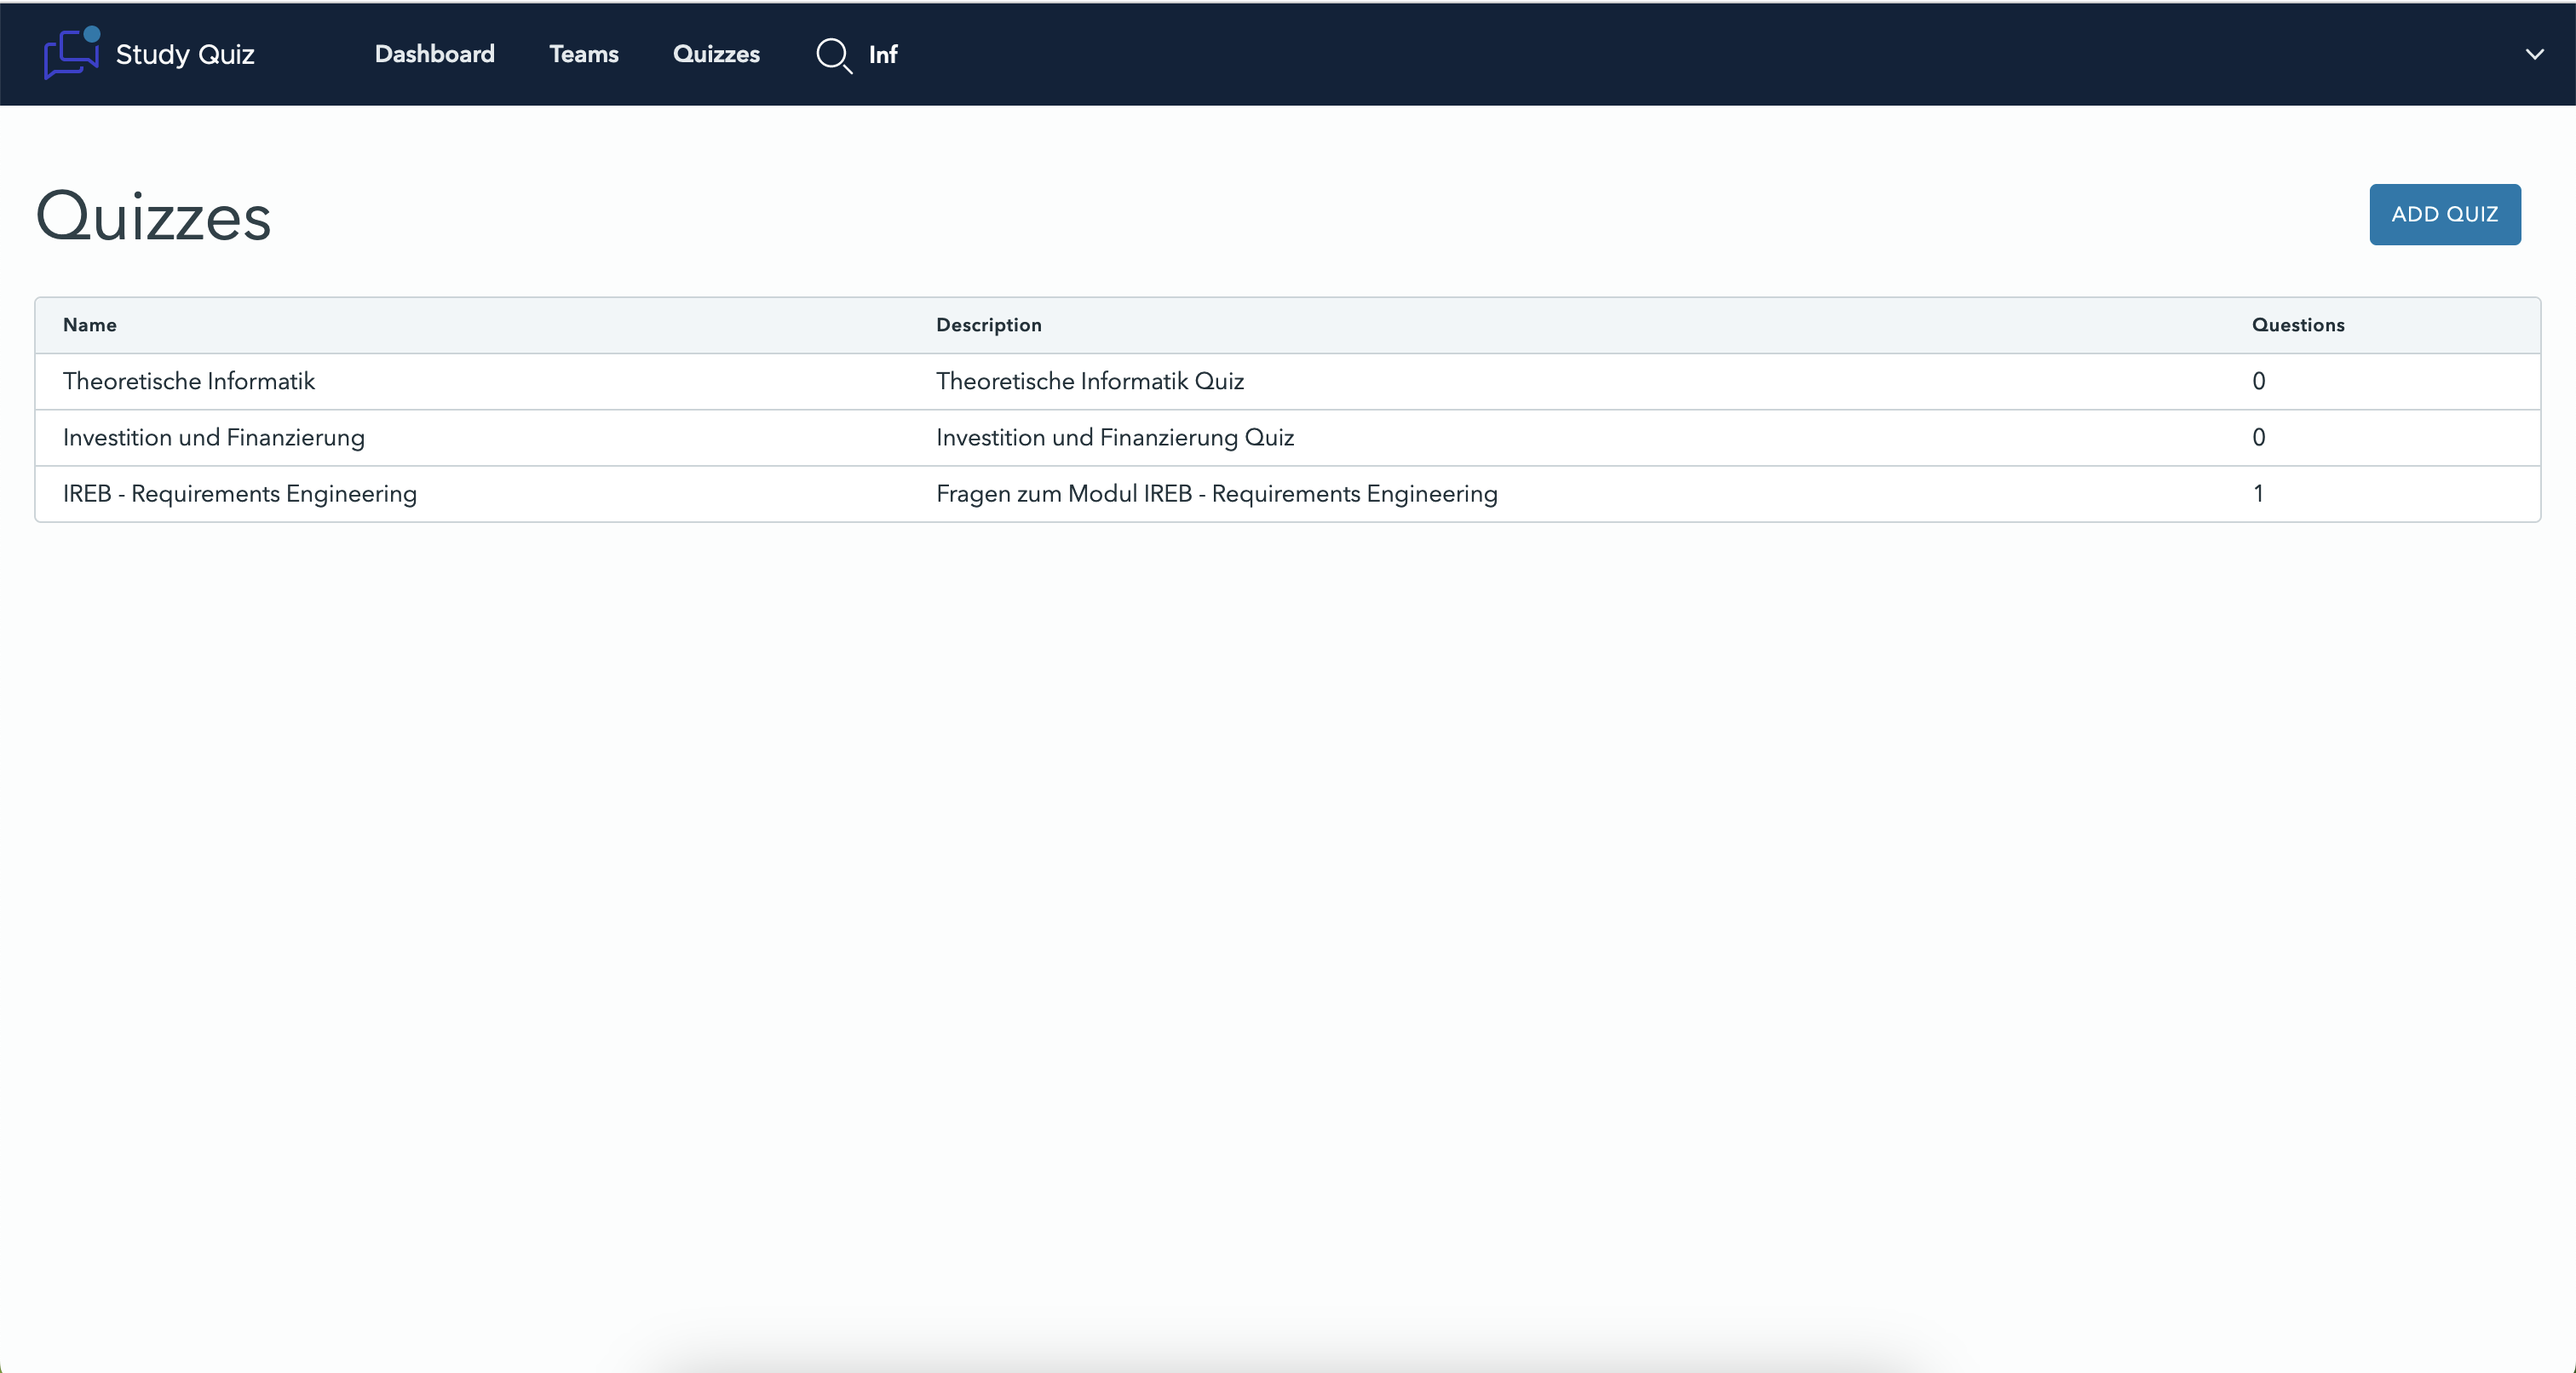
\includegraphics[width=\linewidth]{img/quiz-list.png}
  \caption{Quiz Liste}
  \label{fig:quiz}
\end{figure}

\begin{figure}[H]
  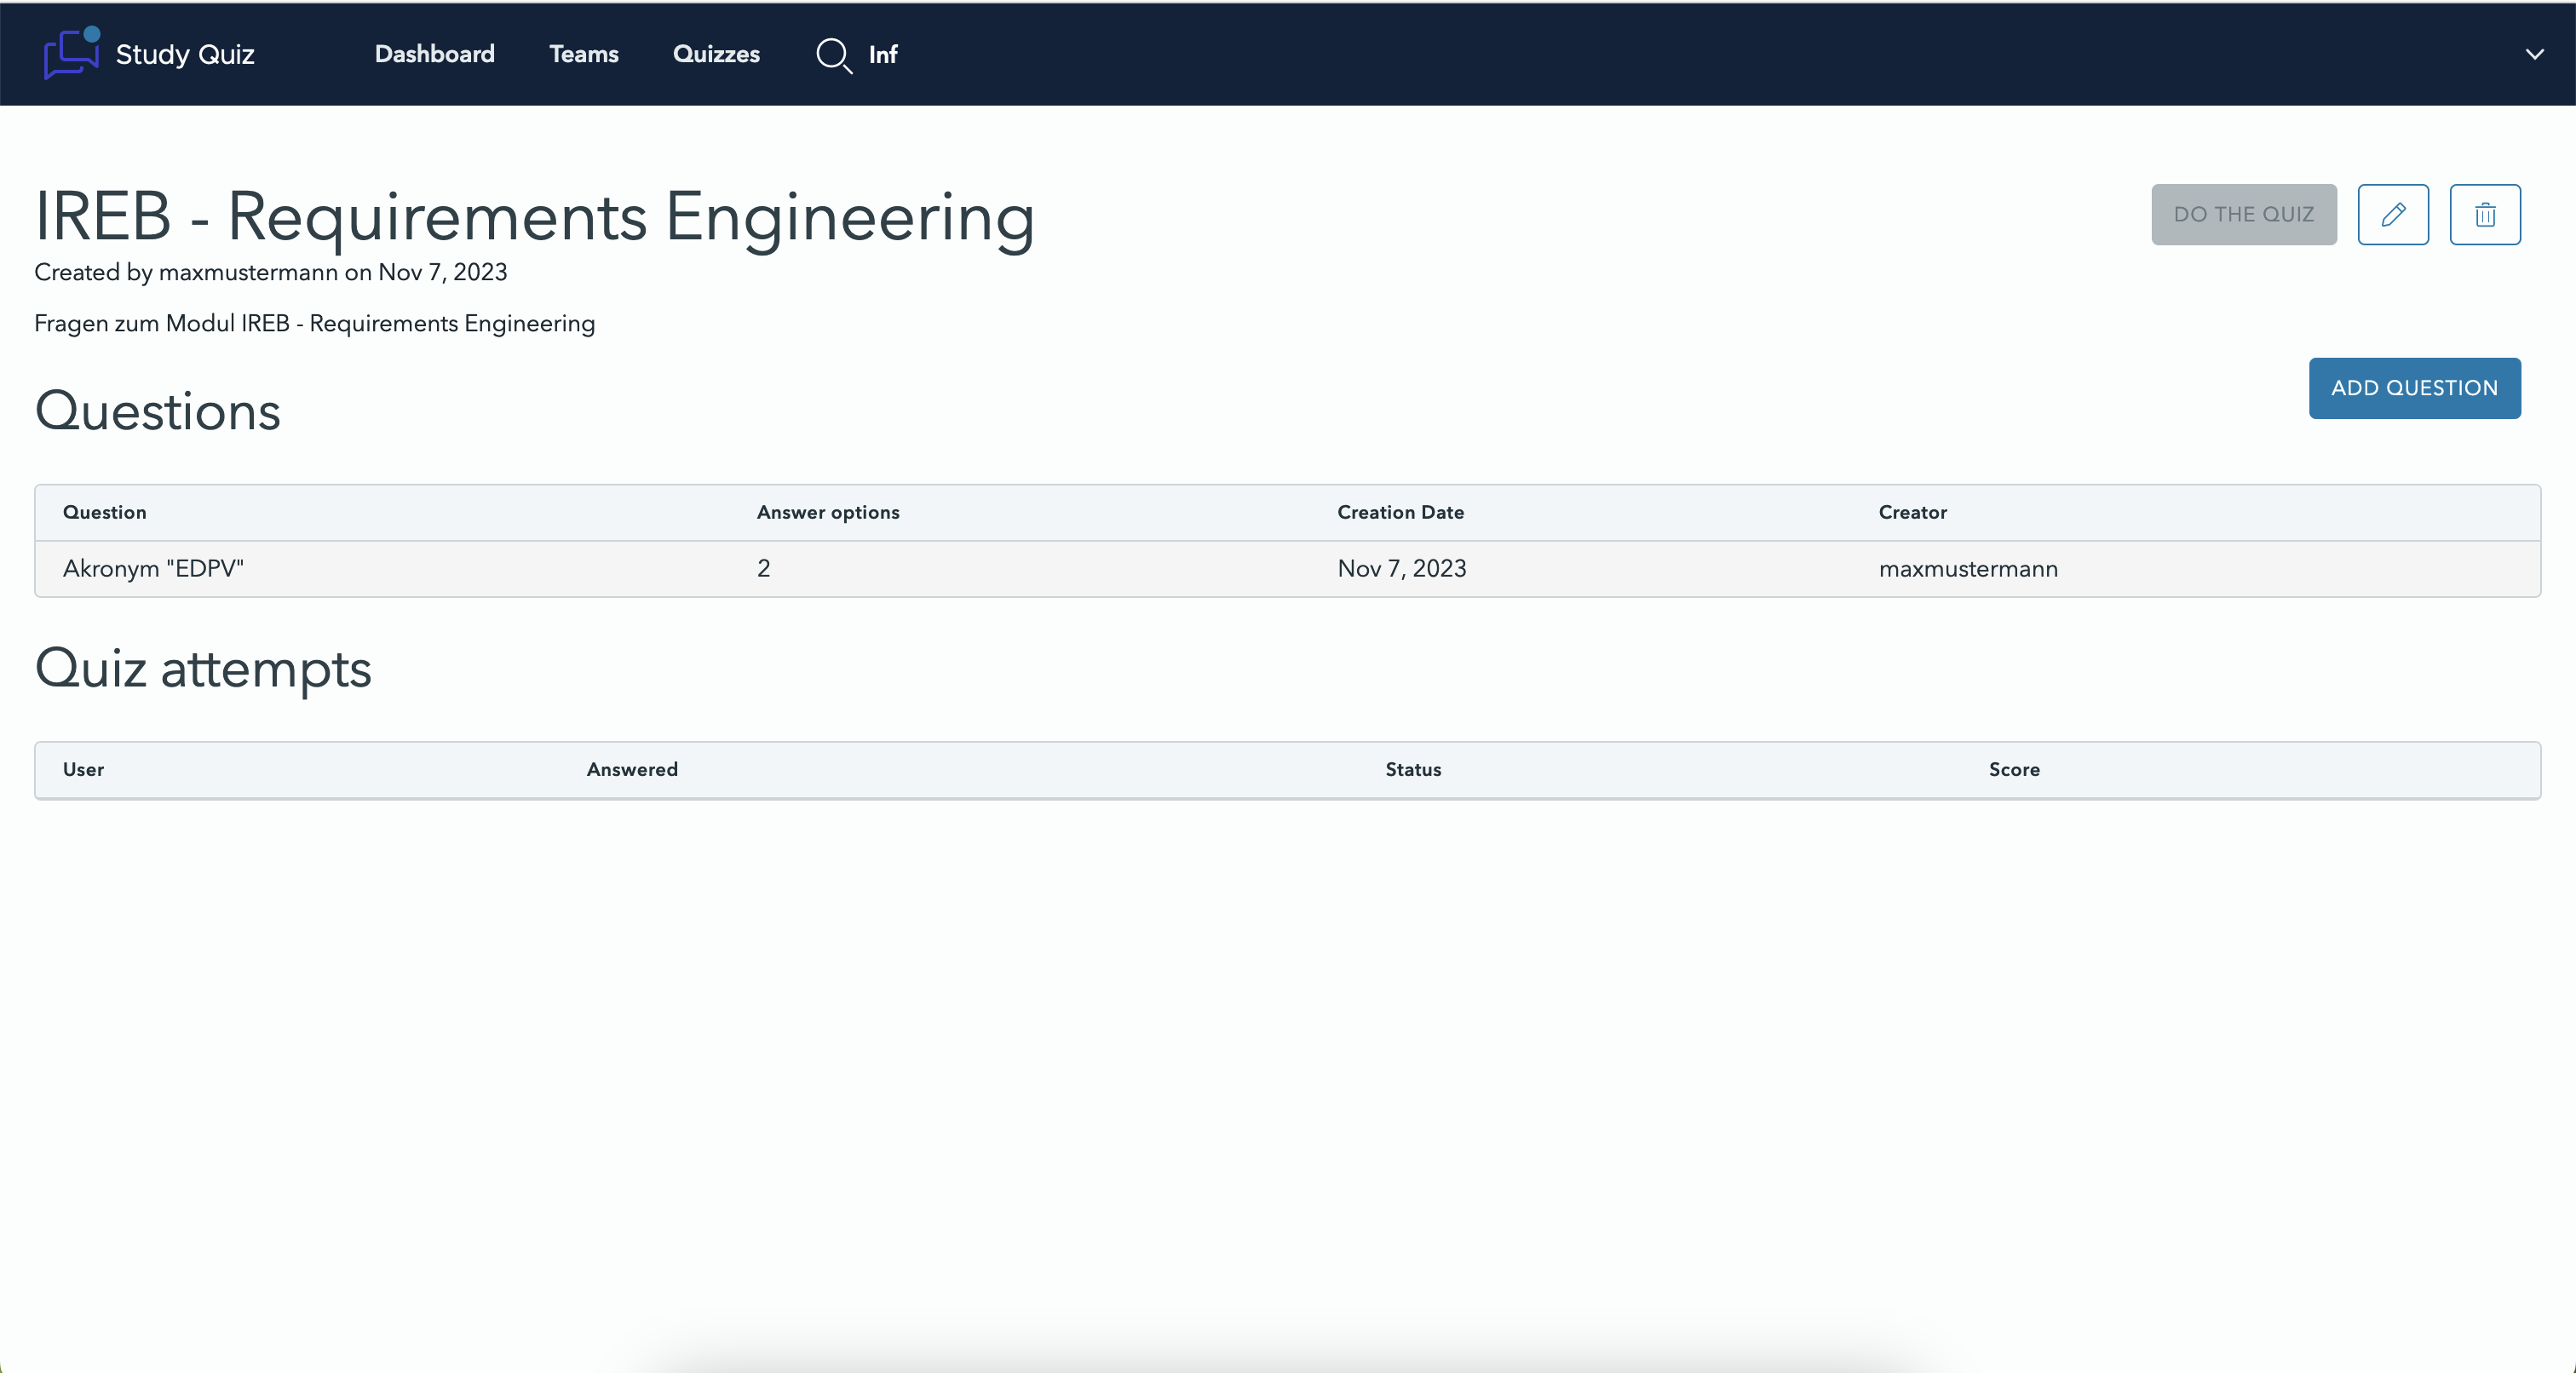
\includegraphics[width=\linewidth]{img/quiz-detail.png}
  \caption{Quiz Übersicht Seite}
  \label{fig:quiz}
\end{figure}

% TODO: Add Do-Quit Page

\subsection*{Team Seiten}

\begin{figure}[H]
  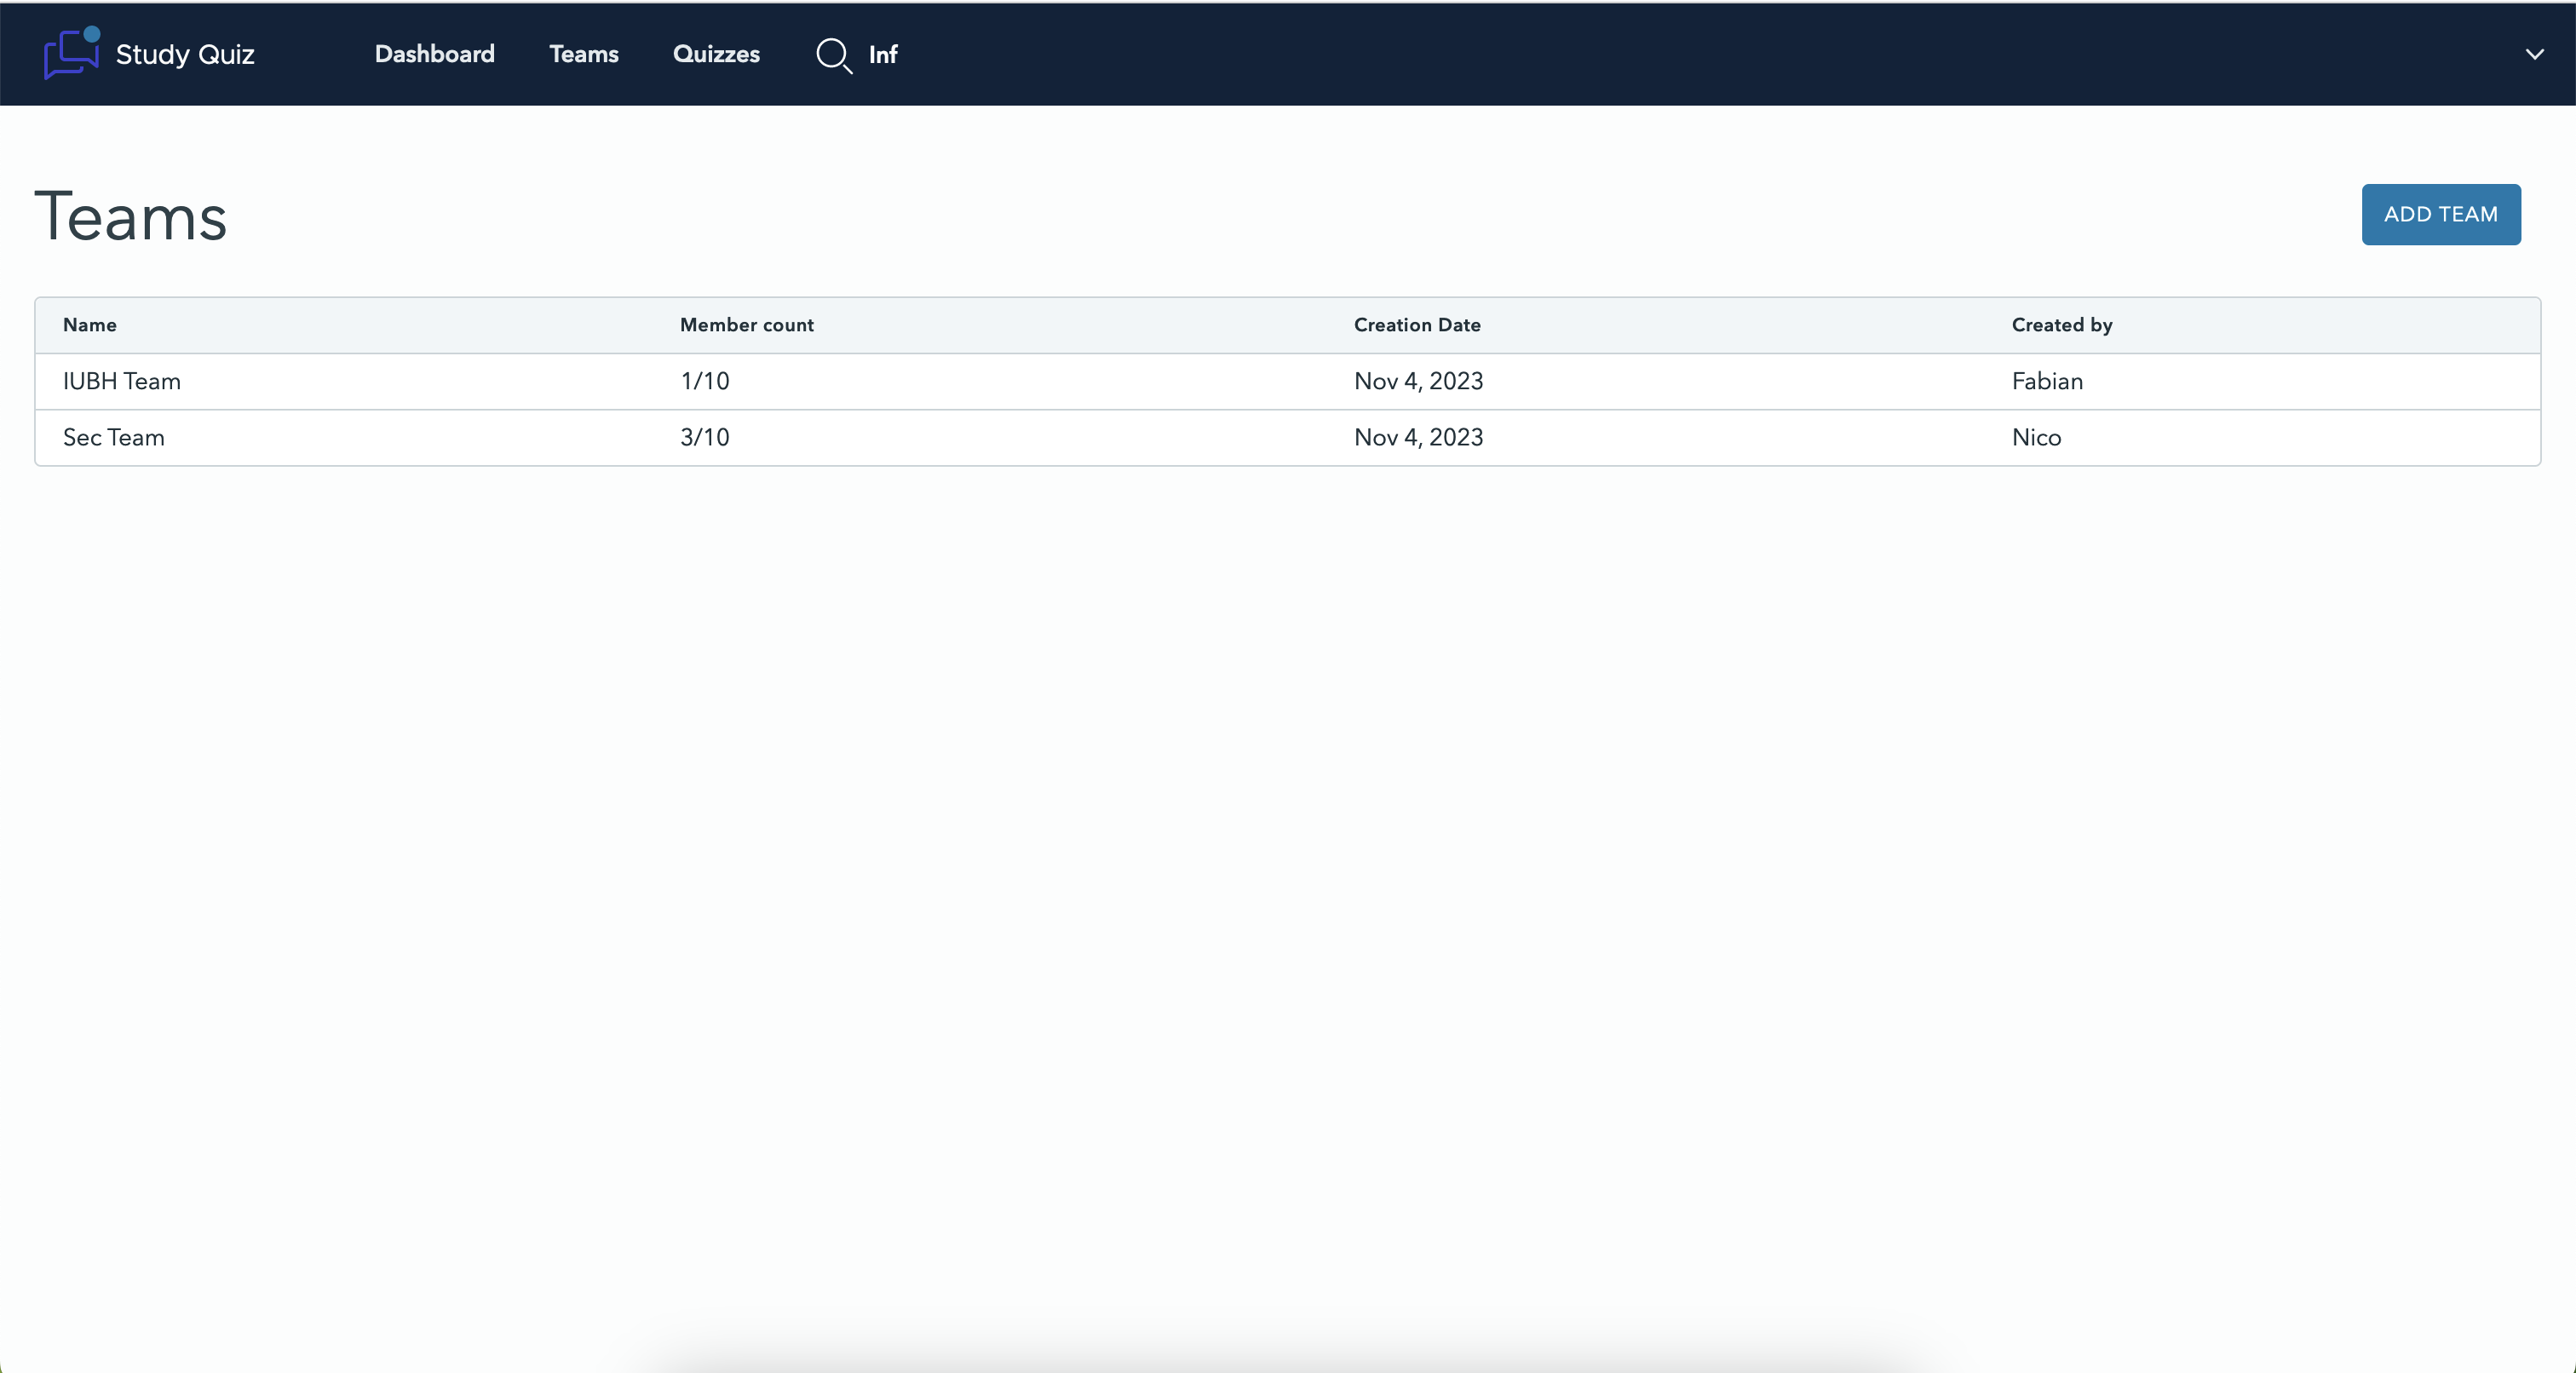
\includegraphics[width=\linewidth]{img/team-list.png}
  \caption{Team Liste}
  \label{fig:team}
\end{figure}

\begin{figure}[H]
  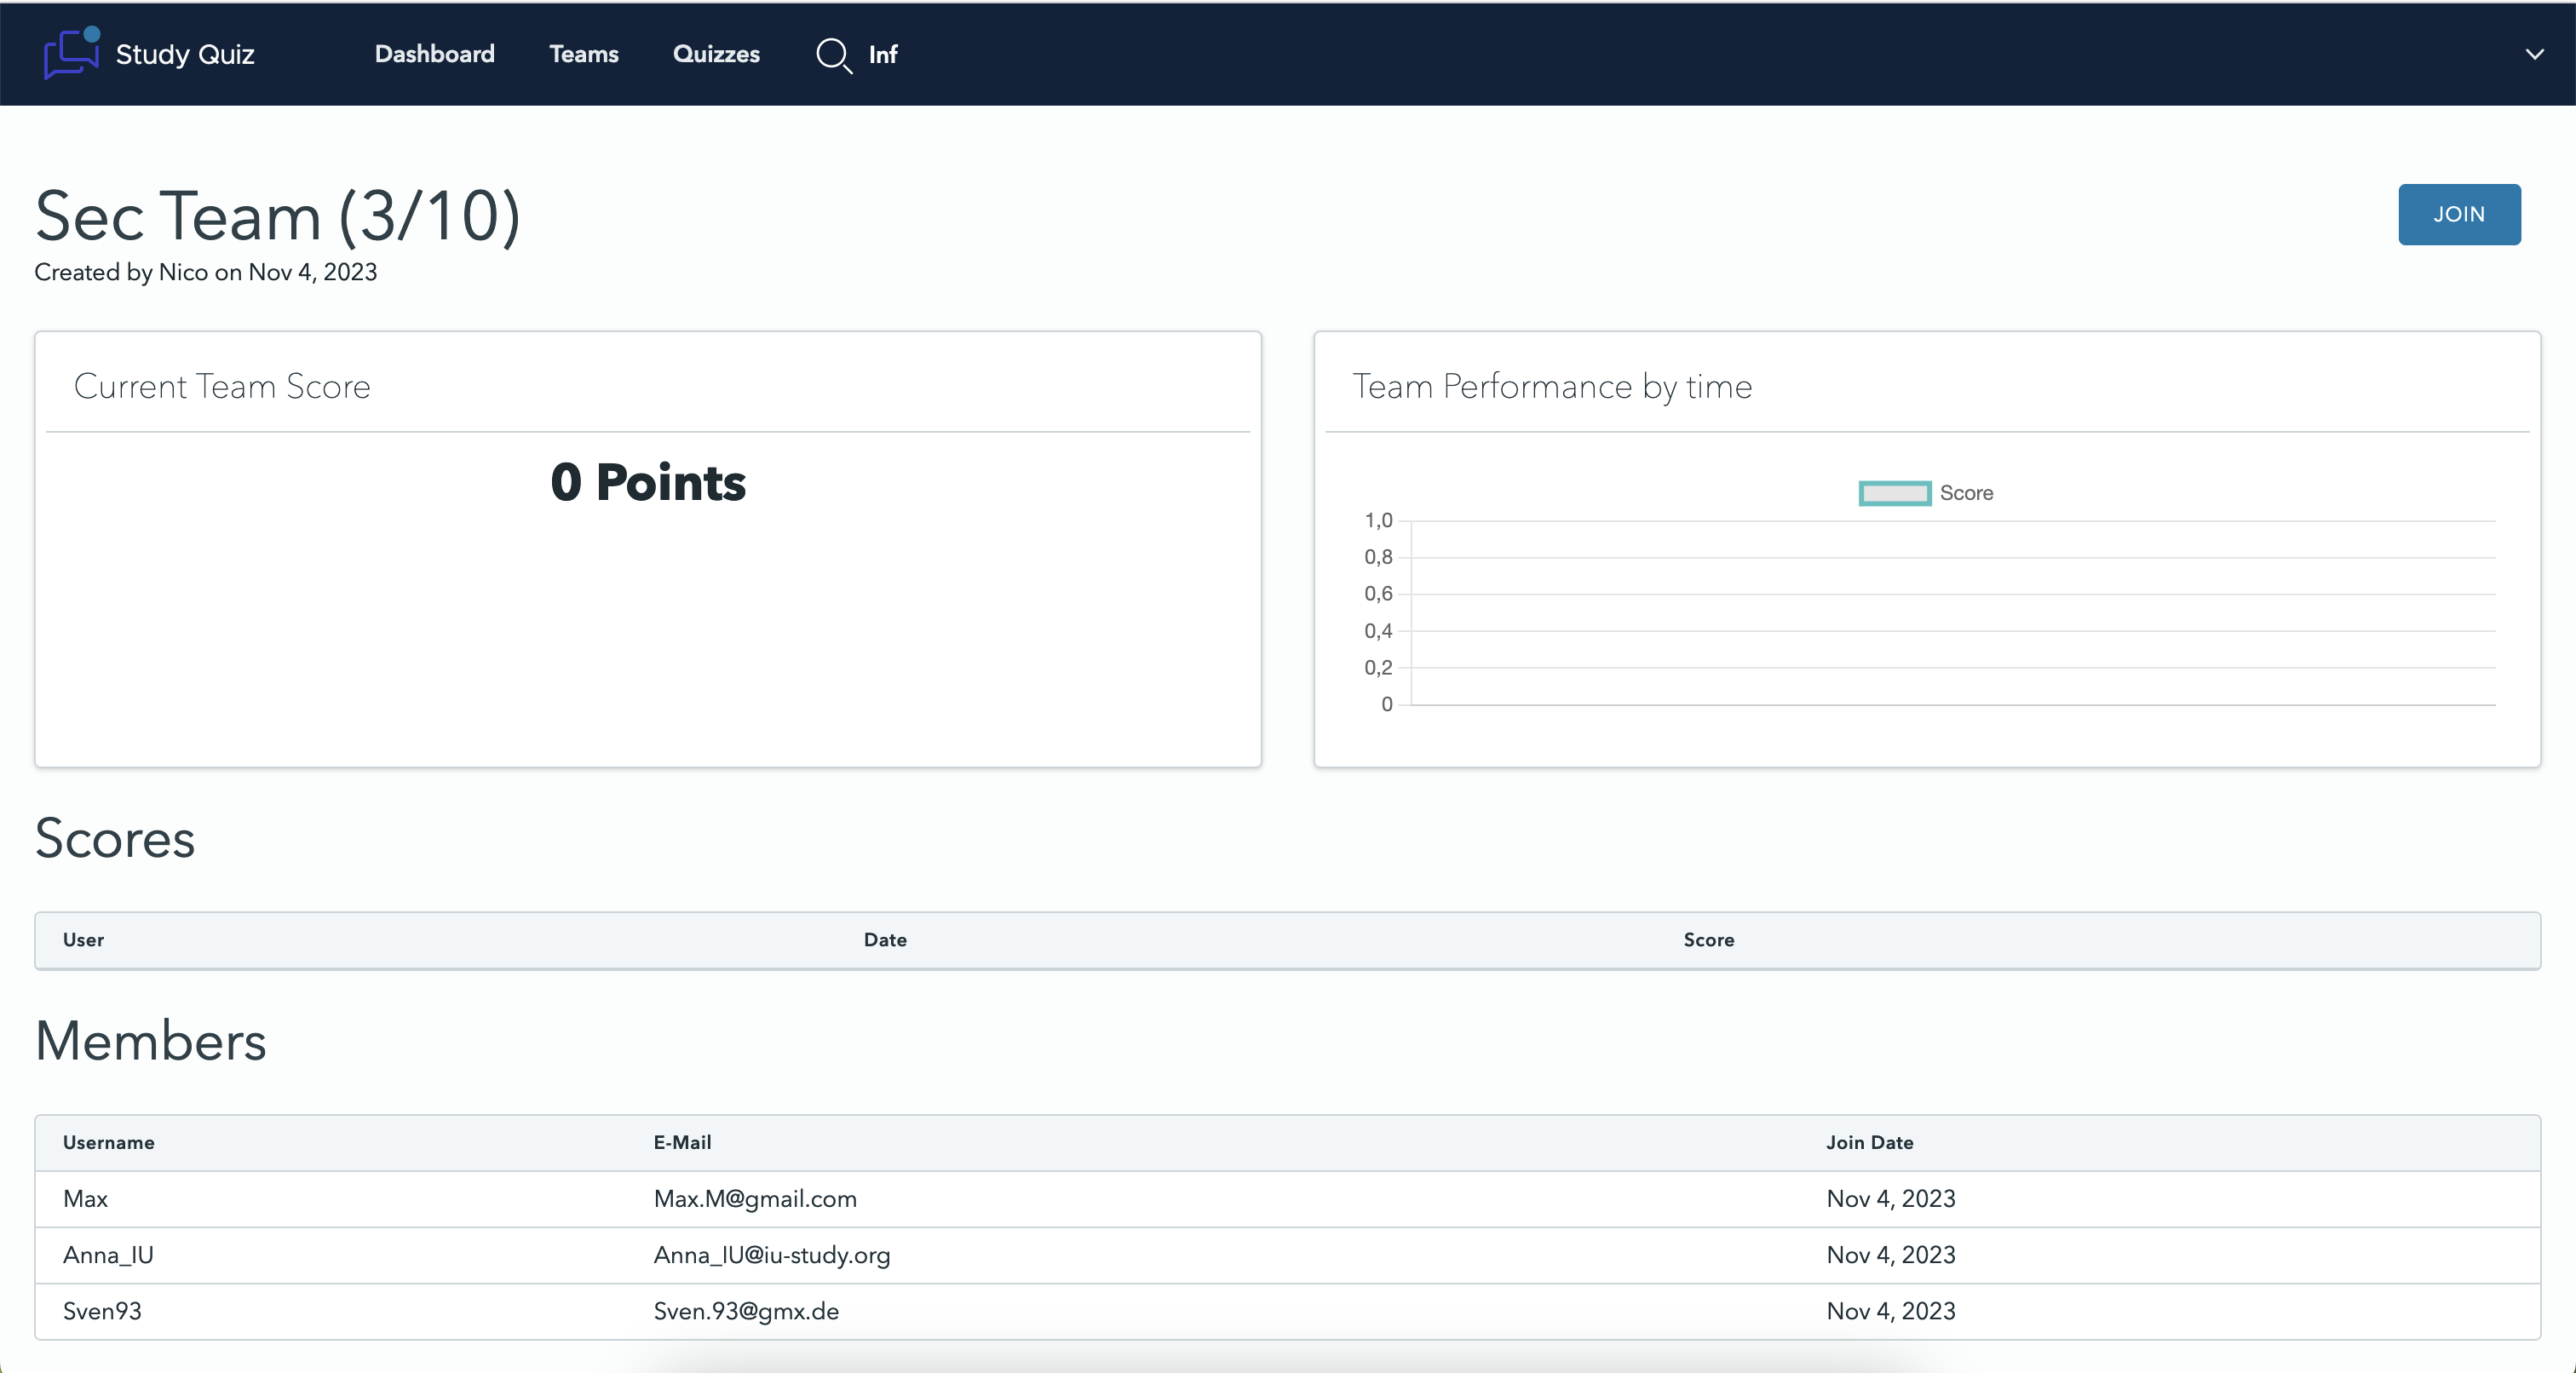
\includegraphics[width=\linewidth]{img/team-detail.png}
  \caption{Team Übersicht Seite}
  \label{fig:team}
\end{figure}
